\documentclass[a4paper,utf8]{article}
\usepackage{rapport}
\usepackage[normalem]{ulem}
\usepackage{amsfonts}
\usepackage{graphicx}
\usepackage{MnSymbol,wasysym}
\usepackage{hyperref}
\usepackage[french]{babel}


\formation{L3MI}
\date{}
\matiere{Conception Orient�e Objet}
\titre{Dots And Boxes - Compte Rendu}

\newcommand\code[1]{\textsf{#1}}
\newcommand\srdjan[1]{{\color{red} #1}}

\begin{document}

\entete

\section{Ce qui a �t� r�alis�}

-Impl�mentation du jeu Puissance 4 en MVC\\%
-Possibilit� de choisir le nombre de lignes et de colonnes\\%
-Possibilit� de changer sa couleur de jeton\\%
-Impl�mentation d\textquotesingle une IA (choix pour chaque joueur si il est humain ou IA)\\%
-Menu de gestion du nombre de joueurs, du type de joueurs (Humain/IA), du nombre de cases. \\%


\section{D�tection des patterns de victoire.}

-Difficult� pour m�moriser quel sont les jetons qui forment le pattern de victoire.

-Difficult� pour l\textquotesingle impl�mentation des diagonales, ci-dessous le sch�ma r�sumant les nombreuses m�thodes de v�rifications.
On a divis� la recherche de diagonale en 4 m�thodes.



On les regroupe ensuite dans une derni�re m�thode qui va se charger de mettre � jour les pions qui ont permis de gagner (en cas de victoire).


\makebox[\textwidth]{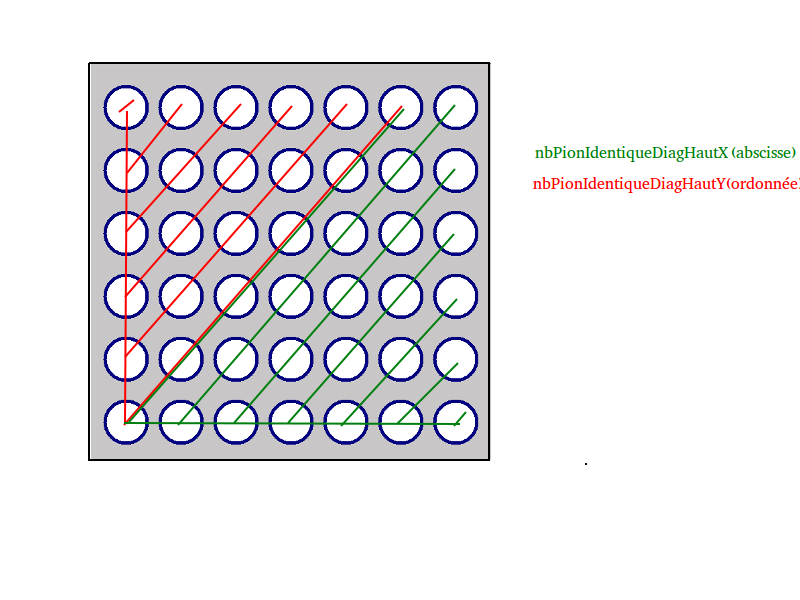
\includegraphics[width=500pt]{img/1}}
\makebox[\textwidth]{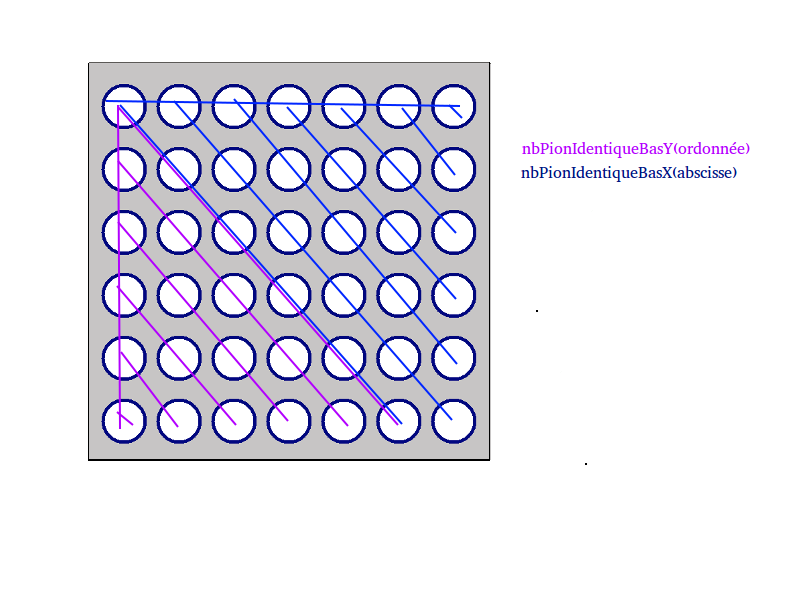
\includegraphics[width=500pt]{img/2}}


\section{M�thode de d�cision de l\textquotesingle IA}


Premi�rement, on va tester pour chaque colonne si le joueur peut gagner.\\%
Si aucune colonne ne permet de gagner, on va regarder o� l\textquotesingle adversaire peut potentiellement gagner et le stopper.\\%
Dans le cas contraire, on va essayer de bloquer l\textquotesingle adversaire au maximum en cherchant la valeur maximum.\\%


\end{document}